\documentclass{article}
\usepackage[backend=biber,citestyle=ieee]{biblatex}
\usepackage[english]{babel}
% \usepackage[swedish]{babel}
\usepackage{graphicx}
\usepackage{csquotes}
\usepackage{float}
\usepackage{datetime}
\usepackage[title]{appendix}
% \usepackage{a4wide} 
\usepackage{amsmath}
\usepackage{subcaption}
\usepackage{textcomp}
\usepackage{gensymb}
\usepackage[font={small},margin={1cm}]{caption}

\usepackage{fancyhdr}   %page header
\pagestyle{fancy}

\usepackage[parfill]{parskip} %Line skip between paragraphs instead of indent

\usepackage{xcolor}
\usepackage{listings}

\input{listings-glsl.prf}

\definecolor{codegreen}{rgb}{0,0.6,0}
\definecolor{codegray}{rgb}{0.5,0.5,0.5}
\definecolor{codepurple}{rgb}{0.58,0,0.82}
\definecolor{backcolour}{rgb}{0.95,0.95,0.95}
\lstdefinestyle{mystyle}{
    backgroundcolor=\color{backcolour},   
    commentstyle=\color{codegreen},
    keywordstyle=\color{magenta},
    numberstyle=\tiny\color{codegray},
    stringstyle=\color{codepurple},
    basicstyle=\ttfamily\footnotesize,
    breakatwhitespace=false,         
    breaklines=true,                 
    captionpos=b,                    
    keepspaces=false,                 
    numbers=left,                    
    numbersep=5pt,                  
    showspaces=false,                
    showstringspaces=false,
    showtabs=false,                  
    tabsize=1
}
\lstset{style=mystyle}

\addbibresource{sources.bib}

\newcommand{\getauthor}{Elias Berglin} %Author
\newcommand{\gettitle}{Labb 3} %Title
\newcommand\norm[1]{\left\lVert#1\right\rVert}

\newdateformat{daymonthyear}{\ordinal{DAY} \monthname[\THEMONTH] \THEYEAR} %Date

\title{\gettitle}
\author{\getauthor}

\date{\daymonthyear\today} %Remove for swedish date

\begin{document}

    % Title 
    \pagenumbering{gobble}
    \maketitle
    \newpage

    % Page header and footer
    \pagenumbering{arabic}
    \fancyhf{}
    \lhead{\getauthor}
    \rhead{\gettitle}
    \rfoot \thepage

    % Document starts here
    \section{Week 5}
    \subsection{Assignment 5}
    \subsubsection{Optical Flow}
    I used OpenCV's implementation for Optical Flow. This was originally used for videos but was adopted to be used with images instead. Coarse-to-fine algorithm improves our result on larger deltas by creating different layers of the image in different sizes. The smaller sizes helps the algorithm find features points. The itterations helps the algorithm to improve our results by correcting errors. In figure \ref{fig:flow-inputs} we can see the input images and in figure \ref{fig:flow-vectors} we can see the different results. We can see that the arrows correct them selves with more iterations and the points getting more accurate with more layers. The Python code can be found in appendix \ref{appendix:OF}

    \begin{figure}[H]
        \centering
        \begin{subfigure}{0.32\textwidth}
            \centering
            \includegraphics[width=1\textwidth]{im1.jpg}
            \caption{First image}
            \label{fig:sub:flow-first-frame}
        \end{subfigure}
        \begin{subfigure}{0.32\textwidth}
            \centering
            \includegraphics[width=1\textwidth]{im2.jpg}
            \caption{Second image}
            \label{fig:sub:flow-second-frame}
        \end{subfigure}  
        \begin{subfigure}{0.32\textwidth}
            \centering
            \includegraphics[width=1\textwidth]{combined.png}
            \caption{Images overlayed}
            \label{fig:sub:flow-combined}
        \end{subfigure} 
        \caption{The two input images for Optical Flow and the the images overlayed} 
        \label{fig:flow-inputs} 
    \end{figure}

    \begin{figure}[H]
        \centering
        \begin{subfigure}{0.48\textwidth}
            \centering
            \includegraphics[width=1\textwidth]{2levels-2iterations.png}
            \caption{2 levels  and 2 iterations}
            \label{fig:sub:flow-low-it-no-pyr}
        \end{subfigure}
        \hspace{5px}
        \begin{subfigure}{0.48\textwidth}
            \centering
            \includegraphics[width=1\textwidth]{2levels-10iterations.png}
            \caption{2 level and 10 iterations}
            \label{fig:sub:flow-low-it}
        \end{subfigure}  
        \begin{subfigure}{0.48\textwidth}
            \centering
            \includegraphics[width=1\textwidth]{3levels-2iterations.png}
            \caption{3 layers and 2 iterations}
            \label{fig:sub:flow-no-pyr}
        \end{subfigure}
        \hspace{5px}
        \begin{subfigure}{0.48\textwidth}
            \centering
            \includegraphics[width=1\textwidth]{3levels-10iterations.png}
            \caption{3 layers and 10 iterations}
            \label{fig:sub:flow}
        \end{subfigure}   
        \caption{Resulting vectors from Lucas-Kanade method with different amount of pyramids and iterations}
        \label{fig:flow-vectors}
    \end{figure}

    \subsubsection{K-means}
    The K-means function can be found in equation \ref{eq:kMeans}. This algorithm assumes that all the datasets belong to a category $\mu$.
    \begin{equation}
        \label{eq:kMeans}
        \min_{\mu, y} \sum_i \norm{x_i - \mu_{y_i}}^2
    \end{equation}

    In figure \ref{fig:kMeansIter} we can see the different iterations. In figure \ref{fig:sub:k0} is the original data categorized. Then first iteration in figure \ref{fig:sub:k1} and then when we compare that to \ref{fig:sub:k2} we see that nothing changes and thus our final categorized are decided. These images were produced with a python script that can be found in appendix \ref{appendix:kmeans}.
    \begin{figure}[H]
        \centering
        \begin{subfigure}{0.32\textwidth}
            \centering
            \includegraphics[width=1\textwidth]{k0.png}
            \caption{0 Iterations}
            \label{fig:sub:k0}
        \end{subfigure}
        \begin{subfigure}{0.32\textwidth}
            \centering
            \includegraphics[width=1\textwidth]{k1.png}
            \caption{1 Iteration}
            \label{fig:sub:k1}
        \end{subfigure}  
        \begin{subfigure}{0.32\textwidth}
            \centering
            \includegraphics[width=1\textwidth]{k2.png}
            \caption{2 Iteration}
            \label{fig:sub:k2}
        \end{subfigure} 
        \caption{Iterations of K-means} 
        \label{fig:kMeansIter} 
    \end{figure}
    \subsubsection{Segmentation}
    I chose to implement K-means for color segmentation. My code can be found in appendix \ref{appendix:color}. Input image can be found in figure \ref{fig:segOri} and output can be found in figure \ref{fig:segOut}. The only parameters I can change is the max number of iterations and the number of clusters. The implementation I created stops the process if 70\% of the clusters have moved less than 1 unit since the last iteration. So the number of max iterations just gives the algorithm more time to reach this criteria. The number of clusters will define how many colors the resulting image will have.

\begin{figure}[H]
    \centering
    \includegraphics[width=1\textwidth]{im1.jpg} 
    \caption{Input for K-means segmentation}
    \label{fig:segOri}
\end{figure}
\begin{figure}[H]
    \centering
    \includegraphics[width=1\textwidth]{segmented.png} 
    \caption{Output from segmentation with 12 clusters and 27 iterations}
    \label{fig:segOut}
\end{figure}

\subsection{Reflections}
I do have much to say other than as usual it was cool to see this different methods in action. The hardest part was to figure out the Coarse-to-fine algorithm and how that improved the optical flow. K-means was just repetition from the data mining course we had. And lastly the coolest thing this week was definitely color segmentation. It was cool to try out different number of clusters to see the different output images.




    \section{Week 6}
    \subsection{Assignment 6}
    \subsubsection{Theory}
    The library I choose for Structure from Motion (SFM) was OpenMVG \cite{moulon2016openmvg}. The library is written in C++ but is run through Python scripts. The Script takes input arguments for both a directory where the input images are located and an output directory. The output consist of a lot of different data. Most importantly it provides a number of .ply files that contain the resulting point cloud. The OpenMVG consists of several submodules for example we have a submodule for running SIFT. To run SFM I used the provided python script, and it goes through the following steps
    \begin{enumerate}
        \item Intrinsic analysis
        \item Feature detection
        \item Feature Matching
        \item Filter Matches
        \item Global Reconstruction
        \item Coloring
    \end{enumerate}

    The first step goes through the metadata of the images extracting the camera sensor that took the image and compares that to a pre-defined database. From this it goes through all the images and extracts data and compiles the necessary data to a JSON file to be used by the rest of the operations.

    \begin{lstlisting}[language=python]
print ("1. Intrinsics analysis")
pIntrisics = subprocess.Popen( [os.path.join(OPENMVG_SFM_BIN, "openMVG_main_SfMInit_ImageListing"),  "-i", input_dir, "-o", matches_dir, "-d", camera_file_params] )
pIntrisics.wait()
    \end{lstlisting}
    Feature detection uses SIFT to extract features from the images and saves the extracted features to files corresponding to the images. 
    \begin{lstlisting}[language=python]
print ("2. Compute features")
pFeatures = subprocess.Popen( [os.path.join(OPENMVG_SFM_BIN, "openMVG_main_ComputeFeatures"),  "-i", matches_dir+"/sfm_data.json", "-o", matches_dir, "-m", "SIFT"] )
pFeatures.wait()
    \end{lstlisting}
    Next we have feature matching and pair generation. The pair generation generates all the possible pairs of images and puts it in a set. The set is then used to pair images and find matches. The matcher file contains multiple matching algorithm, but it prefers to use Cascade Hashing Matcher.

    \begin{lstlisting}[language=python]
print ("3. Compute matching pairs")
pPairs = subprocess.Popen( [os.path.join(OPENMVG_SFM_BIN, "openMVG_main_PairGenerator"), "-i", matches_dir+"/sfm_data.json", "-o" , matches_dir + "/pairs.bin" ] )
pPairs.wait()

print ("4. Compute matches")
pMatches = subprocess.Popen( [os.path.join(OPENMVG_SFM_BIN, "openMVG_main_ComputeMatches"),  "-i", matches_dir+"/sfm_data.json", "-p", matches_dir+ "/pairs.bin", "-o", matches_dir + "/matches.putative.bin" ] )
pMatches.wait()
    \end{lstlisting}
    Next it performes geometric filtering on the matches to filter out bad matches.

    \begin{lstlisting}[language=python]
print ("5. Filter matches" )
pFiltering = subprocess.Popen( [os.path.join(OPENMVG_SFM_BIN, "openMVG_main_GeometricFilter"), "-i", matches_dir+"/sfm_data.json", "-m", matches_dir+"/matches.putative.bin" , "-g" , "f" , "-o" , matches_dir+"/matches.f.bin" ] )
pFiltering.wait()
    \end{lstlisting}
    The last two steps comes down to the actual structure from motion and then coloring the 3D points. The method used here is sequential method. In their library I can see there are three methods for 3D reconstruction. Sequential, Sequential v2 and Global. They provide python script for both sequential and global reconstruction, so that is what I have tried. But I will only look into the sequential part due to the superior result it provided. The codebase for this project is massive, so I will only go through the processing steps.
    \begin{enumerate}
        \item Make sure we have a correct initial pair.
        \item Create an essential matrix from these pairs.
        \item Loop through possible images for reconstruction.
        \begin{enumerate}
            \item Add possible images to reconstruction.
            \item Do bundle adjustment until all points are within a certain precision.
            \item Remove unstable poses and observations.
        \end{enumerate}
        \item Ensure there are no more outliers.
        \item Done
    \end{enumerate}

    \begin{lstlisting}[language=python]
print ("6. Do Sequential/Incremental reconstruction")
pRecons = subprocess.Popen( [os.path.join(OPENMVG_SFM_BIN, "openMVG_main_SfM"), "--sfm_engine", "INCREMENTAL", "--input_file", matches_dir+"/sfm_data.json", "--match_dir", matches_dir, "--output_dir", reconstruction_dir] )
pRecons.wait()

print ("7. Colorize Structure")
pRecons = subprocess.Popen( [os.path.join(OPENMVG_SFM_BIN, "openMVG_main_ComputeSfM_DataColor"),  "-i", reconstruction_dir+"/sfm_data.bin", "-o", os.path.join(reconstruction_dir,"colorized.ply")] )
pRecons.wait()
    \end{lstlisting}

    \subsubsection{Implementation}
    I used openMVG \cite{moulon2016openmvg} and ran both Sequential and Global reconstruction. Due to some errors whit camera calibration when using my own images I used a dataset provided by them with images of Échillais church \cite{ImgDataSet}. Figure \ref{fig:exImg} shows an example of images in the dataset.
    \begin{figure}[H]
        \centering
        \begin{subfigure}{0.48\textwidth}
            \centering
            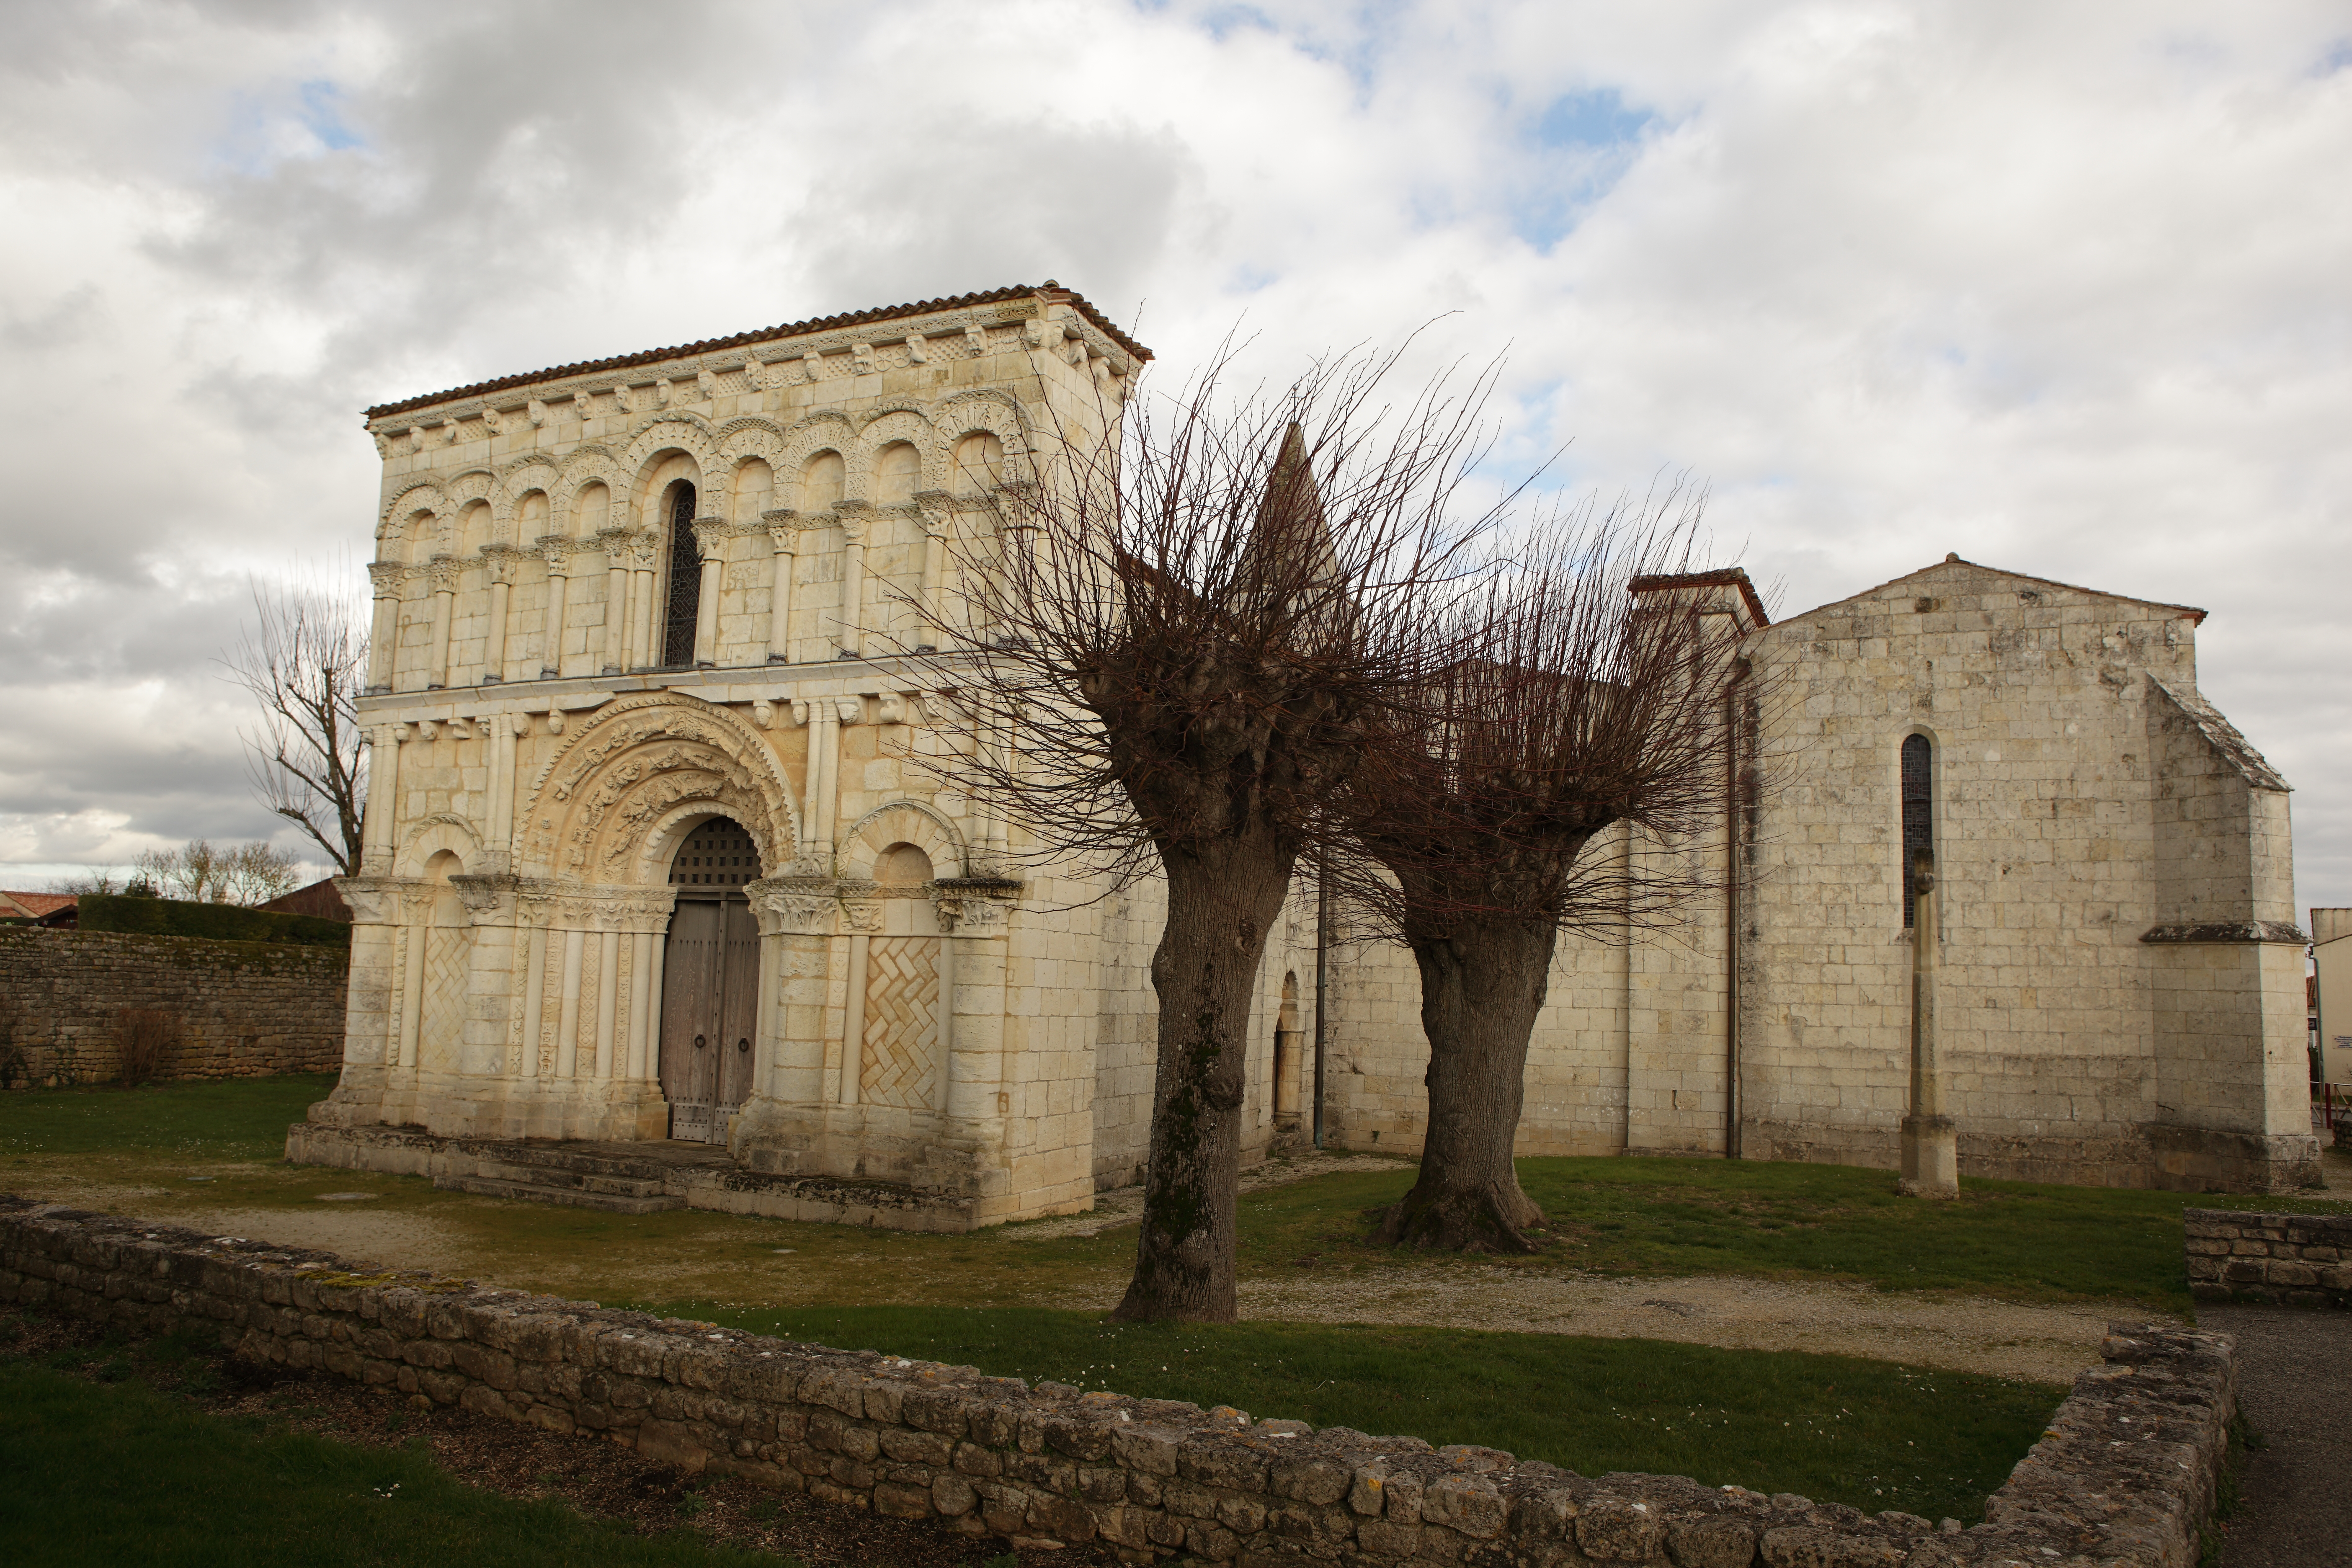
\includegraphics[width=1\textwidth]{ch_img1.JPG}
            \label{fig:sub:exImg1}
        \end{subfigure}
        \hspace{5px}
        \begin{subfigure}{0.48\textwidth}
            \centering
            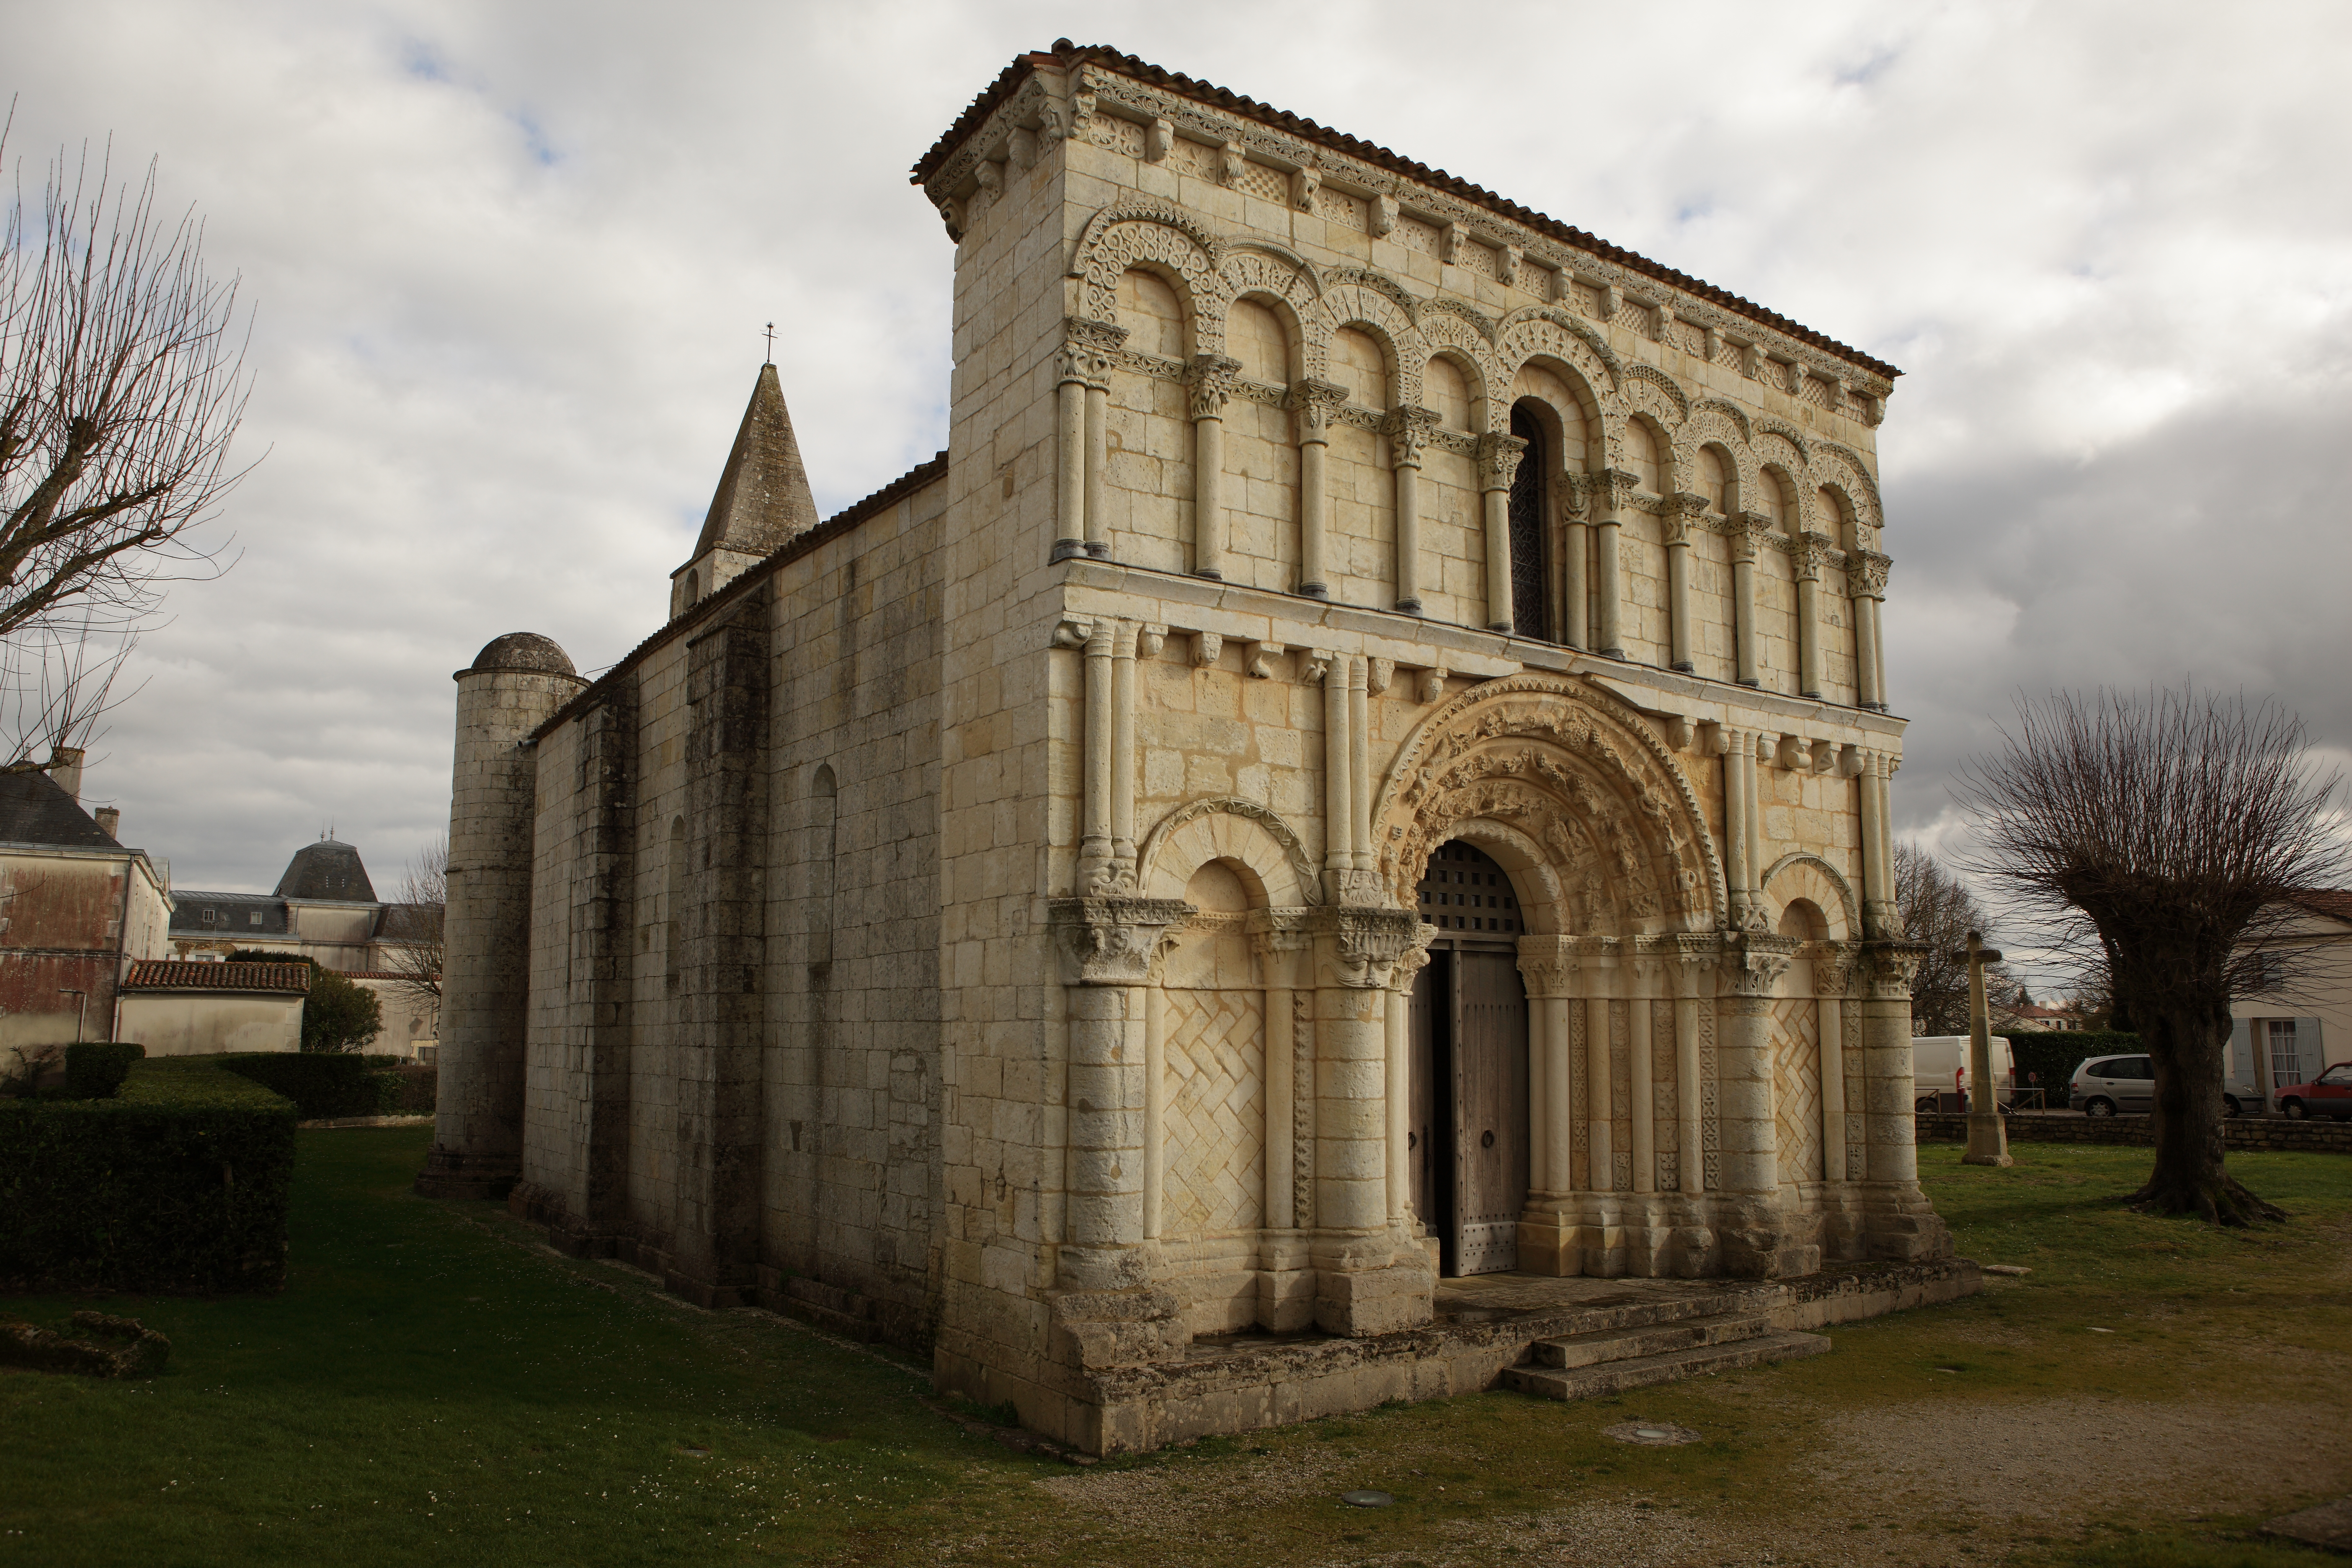
\includegraphics[width=1\textwidth]{ch_img2.JPG}
            \label{fig:sub:exImg2}
        \end{subfigure}  
        \begin{subfigure}{0.48\textwidth}
            \centering
            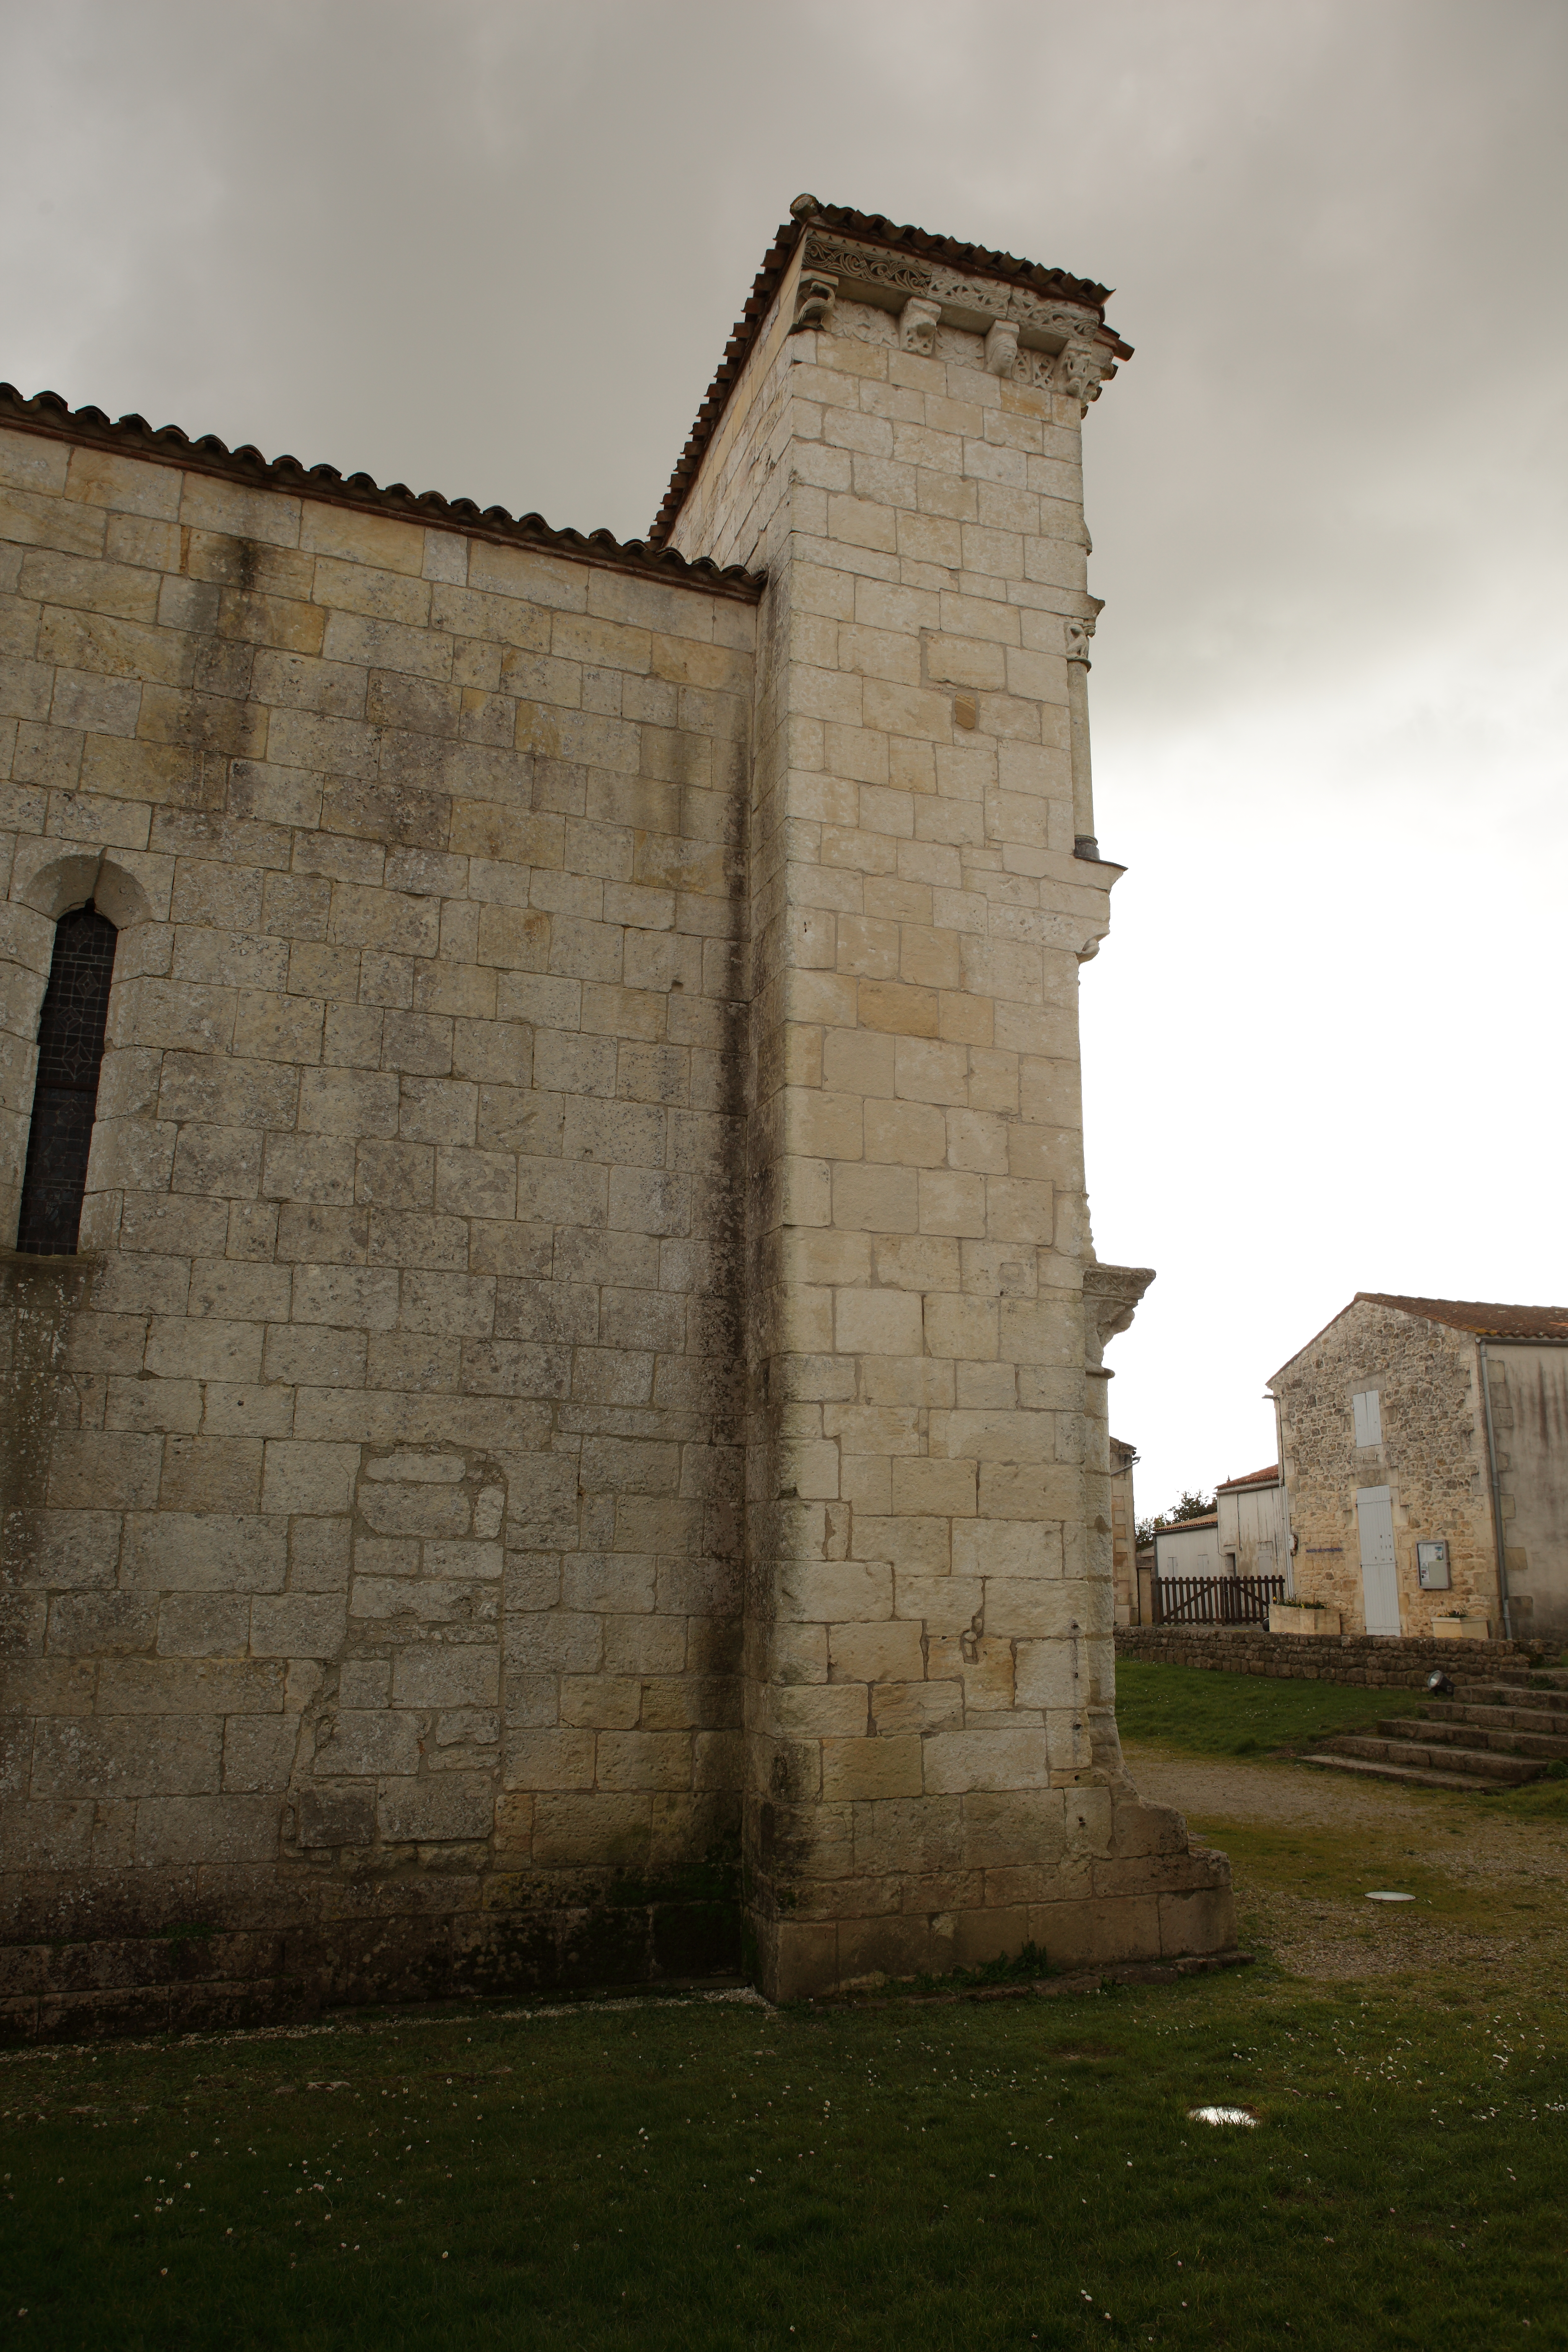
\includegraphics[width=1\textwidth]{ch_img3.JPG}
            \label{fig:sub:exImg3}
        \end{subfigure}
        \hspace{5px}
        \begin{subfigure}{0.48\textwidth}
            \centering
            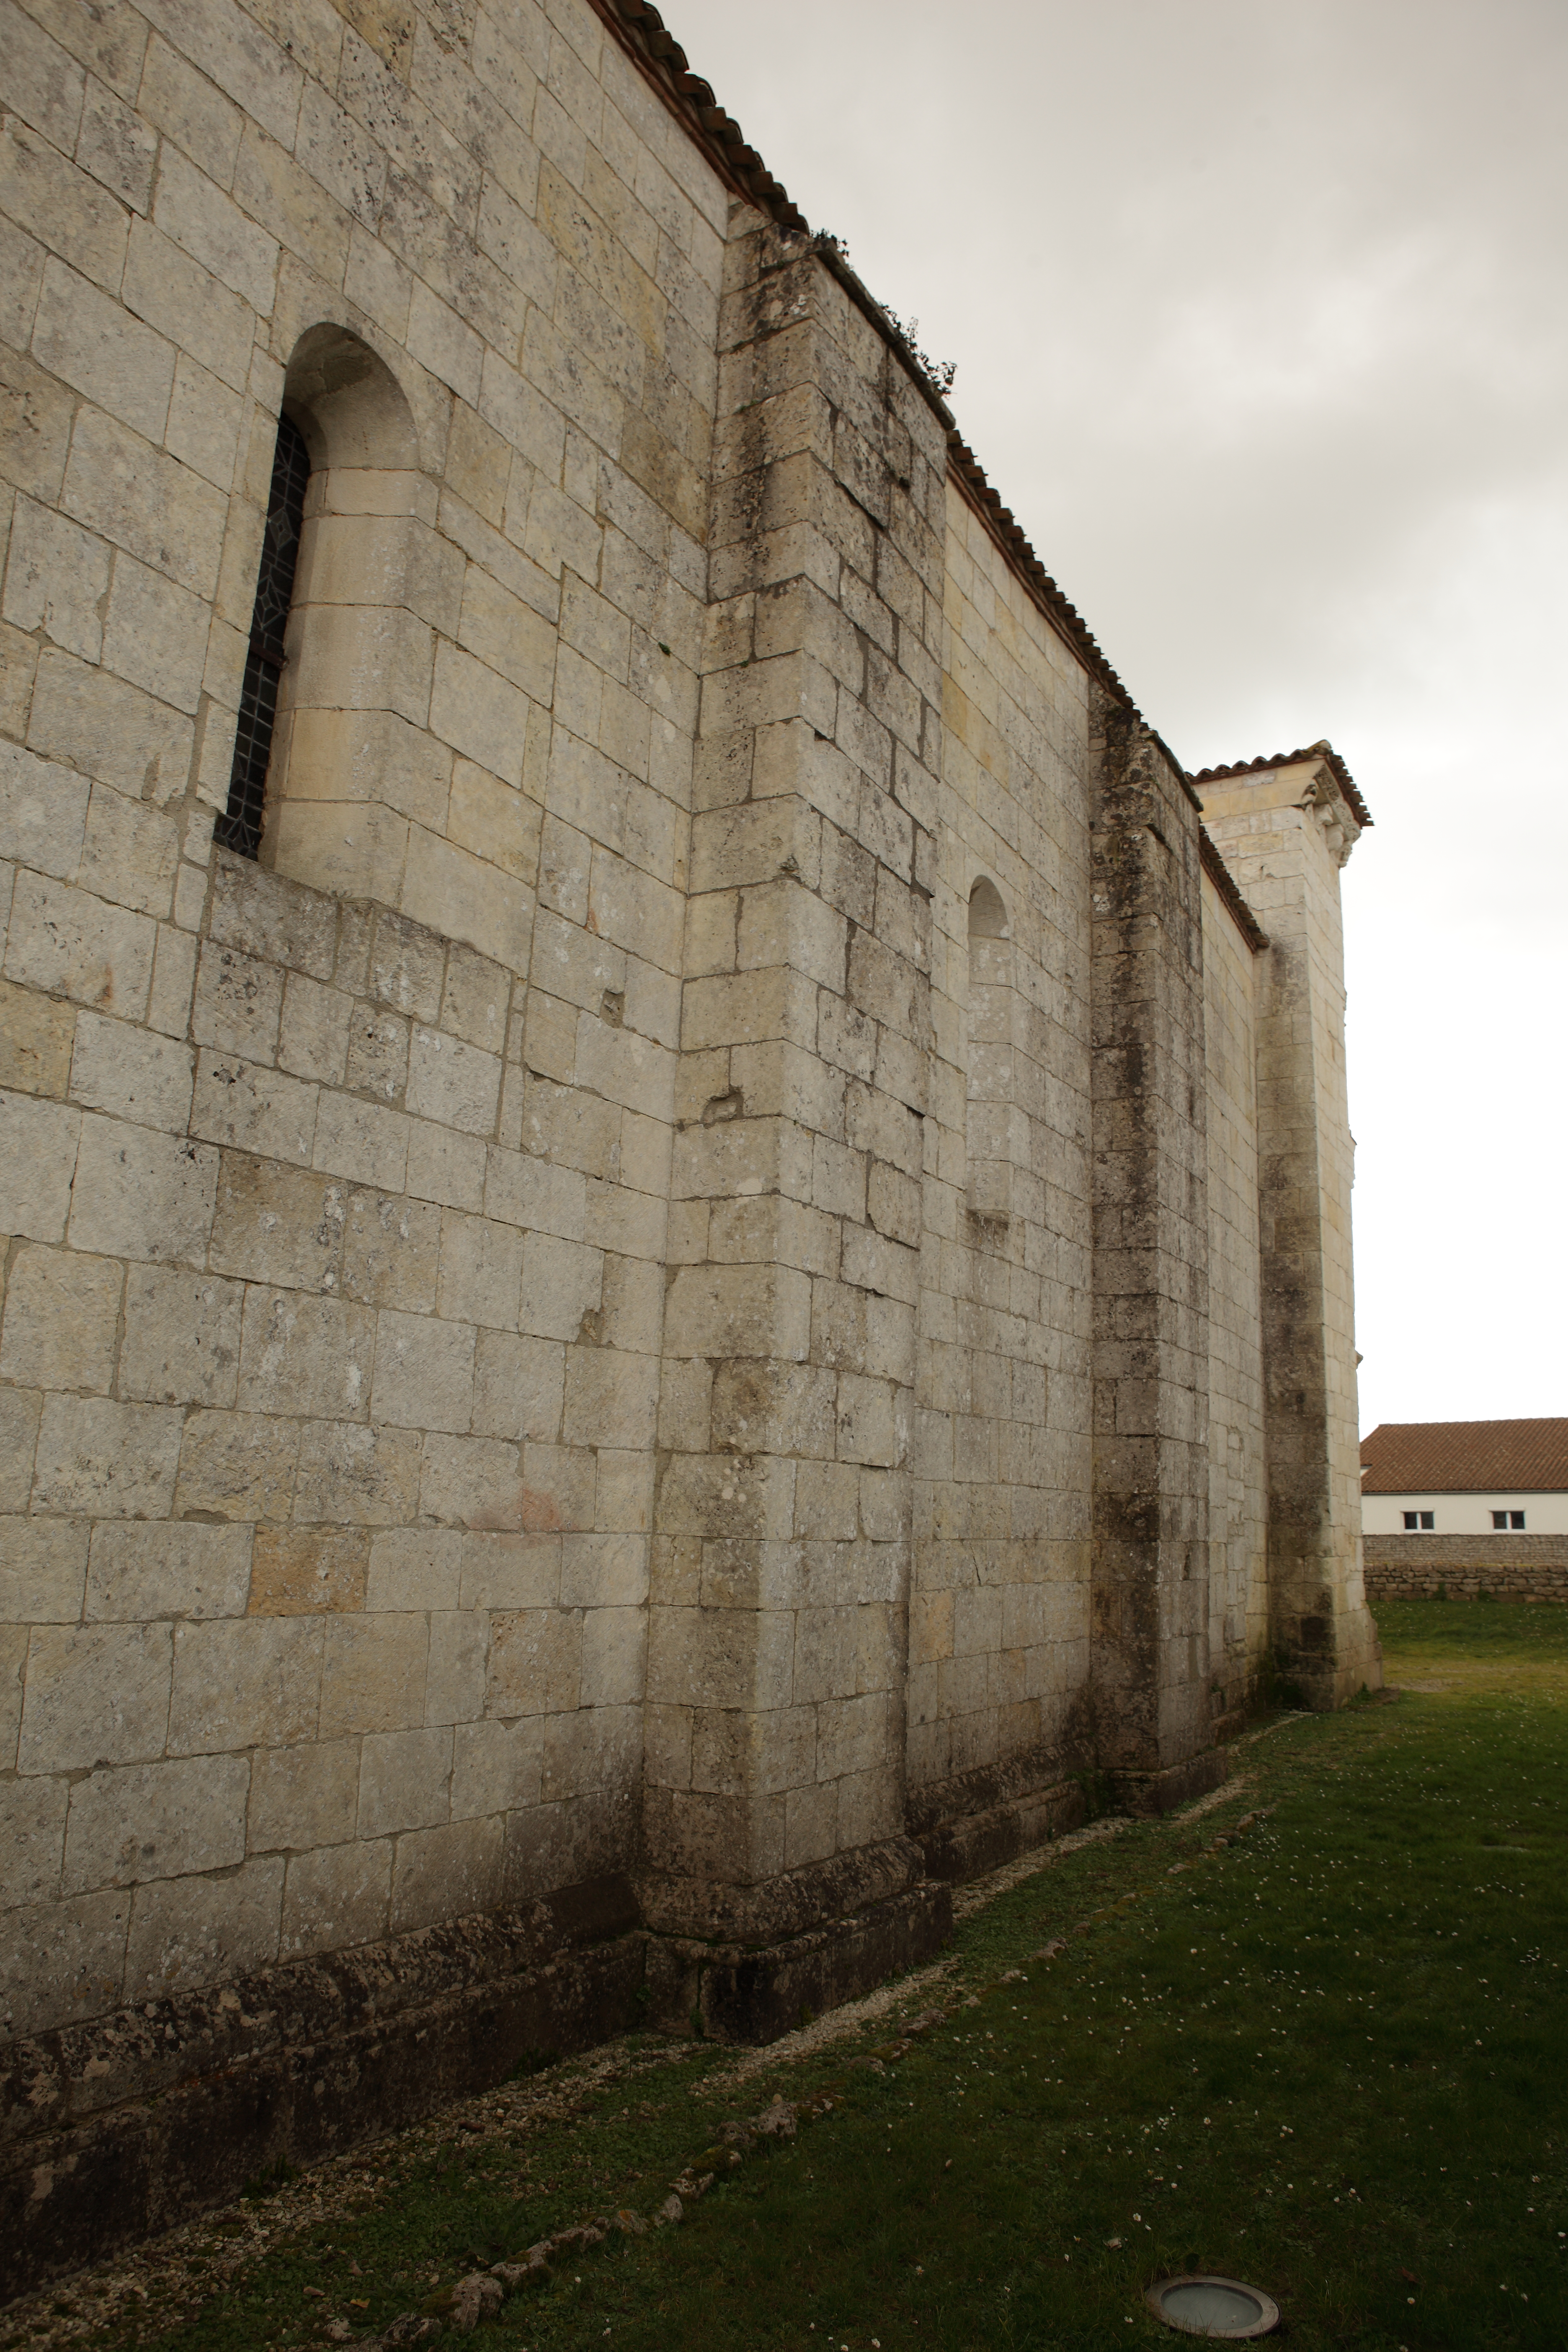
\includegraphics[width=1\textwidth]{ch_img4.JPG}
            \label{fig:sub:exImg4}
        \end{subfigure}   
        \caption{Example images from the Échillais church dataset\cite{ImgDataSet}}
        \label{fig:exImg}
    \end{figure}

    The first reconstruction I did was through the sequential pipeline. The resulting data points are shown in Figure \ref{fig:seqOut}.

\begin{figure}[H]
    \centering
    \includegraphics[width=1\textwidth]{seq_output.png} 
    \caption{Resulting data points from 3D reconstruction using the sequential SFM pipeline}
    \label{fig:seqOut}
\end{figure}

To compare the different pipelines I also ran the global reconstruction pipeline and the resulting data points ca be found in figure \ref{fig:globOut}.

\begin{figure}[H]
    \centering
    \includegraphics[width=1\textwidth]{glob_output.png} 
    \caption{Resulting data points from 3D reconstruction using the sequential SFM pipeline}
    \label{fig:globOut}
\end{figure}

The global pipeline manages to produce is close to the sequential, but it is not as detailed as the sequential pipeline. The easiest way to see this is to look at the tower of the church as it is more detailed on the sequential pipeline.

\subsection{Reflections}
This week I would say was the most interesting week of them all. It was really cool to see how we can use all the previous week's theory into something as cool as Structure from motion. It was hard to found a library that was both easy to understand and could produce a good output. The simplest project I found was a simple python project by Harish Venkataraman \cite{SFMGit}. It had problems with the provided dataset and I could not get it working with my own images. I tried another library called open SFM written in both C++ and python, but I could not get it compiling. 

So I ended up on OpenMVG written i C++ but can be accessed through python. The problem here is I could not get it working with my own images, but it worked flawlessly with their recommended dataset. I got the error down to the library not being able to derive the focal length for my camera. I tried to provide it myself but with no success. In the end I just used their dataset and I think that is for the better due to the "cool factor" of their data set. From one of the provided datasets I was able to reconstruct a church from France and when loaded I could easily see the structure, and it was really cool. 

\section{Week 7}
\subsection{Assignment 7}
\subsubsection{Triangle}
The triangle I choose to do had the following points:
\begin{enumerate}
    \item (3,2)
    \item (2,5)
    \item (7,3)
\end{enumerate}
I then chose the inside point (3,2) and the outside point (2,1). I created a python script to calculate my points. The script can be found in appendix \ref{appendix:tri}. And the plotted result can be found in figure \ref{fig:tri}.

\begin{figure}[H]
    \centering
    \includegraphics[width=1\textwidth]{tri.png} 
    \caption{Resulting data points from 3D reconstruction using the sequential SFM pipeline}
    \label{fig:tri}
\end{figure}

\subsubsection{Phong lighting}
I used python to plot the model. The resulting plot can be seen in figure \ref{fig:pho} and the code can be found in appendix \ref{appendix:pho}. The equation for phong lighting can be found in equation \ref{eq:pho}.

\begin{equation}
    \label{eq:pho}
    I=k_AI_a + k_DI_D+k_S(cos(\varphi))^\alpha I_L
\end{equation}

The fixed value used can be found below:
\begin{itemize}
    \item Light:
    \begin{itemize}
        \item $I_A = 0.3$
        \item $I_D = 0.2$
        \item $I_L = 1.2$
    \end{itemize}
    \item Material:
    \begin{itemize}
        \item $K_A = 0.1$
        \item $K_D = 0.1$
        \item $K_S = 1.0$ 
    \end{itemize}
    \item Variable values
    \begin{itemize}
        \item $(0 \leq \alpha \leq 20) \vee 3 $
        \item $(0 \leq \varphi \leq \frac{\pi}{2}) \vee \frac{\pi}{4}$
    \end{itemize}
\end{itemize}


\begin{figure}[H]
    \centering
    \includegraphics[width=1\textwidth]{phong.png} 
    \caption{Plot of Phong lighting, blue/left is plot based on $\alpha$ and green/right is plot based on $\varphi$}
    \label{fig:pho}
\end{figure}

\subsubsection{Shading}
Python code for creating the 3D image can be found in appendix \ref{appendix:3dCode}. The vertex shader applied can be found in appendix \ref{appendix:vertex} and the fragment shader can be found in appendix \ref{appendix:fragment}. I chose to render a sphere and the final render can be found in figure \ref{fig:sphere}.

\begin{figure}[H]
    \centering
    \includegraphics[width=1\textwidth]{sphere.png} 
    \caption{Final rendered 3D image with lambertian shader}
    \label{fig:sphere}
\end{figure}

\subsection{Reflections}
As always an interesting week. I did however miss this week's lecture. Thankfully I could easily understand the lecture slides and was able to use them to understand Phong,Lambertian and the formula to check if a pixel is within a triangle. The only real problem I encountered this week was the recommended 3D library for python. The first problem was that OpenGL was deprecated on Mac I solved this by using my Windows desktop pc instead. The next problem was due to the fact that Ratcave was no longer in development it had problems with newer version of Scipy which it depended on. This was solved by downgrading the Scipy version to 1.3.3.


    % Sources
    \newpage
    \printbibliography

    % Appendices
    \newpage
    \begin{appendices}

        \section{Python code for optical flow}
        \label{appendix:OF}
        \begin{lstlisting}[language=Python]
import numpy as np
import cv2
import os

frame1 = cv2.imread("im1.jpg")
frame2 = cv2.imread("im2.jpg")

frame1g = cv2.cvtColor(frame1, cv2.COLOR_BGR2GRAY)
frame2g = cv2.cvtColor(frame2, cv2.COLOR_BGR2GRAY)

combined = cv2.addWeighted(frame1, 0.3, frame2, 0.5, 0)
cv2.imwrite("pyramid/combined.png", combined)

parameters = dict(maxCorners=100, qualityLevel=0.3, minDistance=7, blockSize=7)

p0 = cv2.goodFeaturesToTrack(frame1g, mask=None, **parameters)

maxLevels = [2,3]
maxIterations = [2, 10]

for level in maxLevels:
    print("On Max Level: ", level)
    for iter in maxIterations:
        OFparams = dict(
            winSize=(15, 15),
            maxLevel=level,
            criteria=(cv2.TERM_CRITERIA_EPS |
                      cv2.TERM_CRITERIA_COUNT, iter, 0.03),
        )
        p1, st, err = cv2.calcOpticalFlowPyrLK(
            frame1g, frame2g, p0, None, **OFparams)
        good_new = p1[st == 1]
        good_prev = p0[st == 1]

        arrows = np.zeros_like(combined)

        for i, (n, p) in enumerate(zip(good_new, good_prev)):
            nx, ny = n.ravel()
            px, py = p.ravel()

            nx = int(nx)
            ny = int(ny)
            px = int(px)
            py = int(py)

            arrows = cv2.arrowedLine(arrows, (px, py), (nx, ny), [
                                     255, 0, 255], 2, cv2.LINE_AA, tipLength=0.4)

            output = cv2.add(combined, arrows)
            if(not os.path.exists("pyramid/"+str(level))):
                os.mkdir("pyramid/"+str(level))
            outName = "pyramid/" + str(level)+"/" + \
                str(level) + "levels-" + str(iter)+"iterations.png"
            cv2.imwrite(outName, output)

        \end{lstlisting}
        \section{K-means}
        \label{appendix:kmeans}
        \begin{lstlisting}[language=python]
from typing import Tuple
from typing import List
import matplotlib.pyplot as plt
from numpy import sqrt
import numpy as np

def centerToLists(center1, center2):
    return ([center1[0], center2[0]], [center1[1], center2[0]])


def drawPlot(center1, center2, gc1, gc2):
    plt.scatter([i[0] for i in gc1], [i[1] for i in gc1], c='blue')
    plt.scatter([i[0] for i in gc2], [i[1] for i in gc2], c='red')
    plt.scatter(center1[0], center1[1],c='lightblue')
    plt.scatter(center2[0], center2[1],c='orange')

def calcDistance(p1, p2):
    return sqrt((p1[0] -p2[0])**2 + (p1[1] - p2[1])**2)

def categorizePoints(points, center1, center2) -> Tuple[List, List]:
    gc1 = []
    gc2 = []
    for point in points:
        d1 = calcDistance(point, center1)
        d2 = calcDistance(point, center2)
        if d1 < d2:
            gc1.append(point)
        else:
            gc2.append(point)
    return (gc1, gc2)

def calculateNewCenter(gc1: List, gc2: List) -> Tuple[Tuple, Tuple]:
    g1x = np.asarray([i[0] for i in gc1]).sum()/len(gc1)
    g1y = np.asarray([i[1] for i in gc1]).sum()/len(gc1)

    g2x = np.asarray([i[0] for i in gc2]).sum()/len(gc2)
    g2y = np.asarray([i[1] for i in gc2]).sum()/len(gc2)

    return ((g1x, g1y), (g2x, g2y))
    


points = [
    (0, 0.5),
    (0, 0.75),
    (1, 1),
    (1.1, 0.4),
    (1, 5, 0.75),
    (2.5, 1),
    (3, 2),
    (4, 1.5),
    (4, 2.5),
    (5, 2)
]

center1 = (1,1.5)
center2 = (3,1)

(gc1, gc2) = categorizePoints(points, center1, center2)
drawPlot(center1, center2, gc1, gc2)
plt.show()
(center1, center2) = calculateNewCenter(gc1, gc2)
(gc1, gc2) = categorizePoints(points, center1, center2)
drawPlot(center1, center2, gc1, gc2)
plt.show()
(center1, center2) = calculateNewCenter(gc1, gc2)
(gc1, gc2) = categorizePoints(points, center1, center2)
drawPlot(center1, center2, gc1, gc2)
plt.show()





        \end{lstlisting}
        \section{Color segmentation}
        \label{appendix:color}
        \begin{lstlisting}[language=python]
import numpy as np
import cv2
from typing import List, Tuple
import collections
import random
import math
from PIL import Image

class Point:
    position = (0,0)
    color = [0,0,0]
    category = [0,0,0]


def convImForShow(im):
    return cv2.cvtColor(im, cv2.COLOR_RGB2BGR)

def calcDistance(p1, p2) -> float:
    x = np.square(p1[0] - p2[0])
    y = np.square(p1[1] - p2[1])
    z = np.square(p1[2] - p2[2])
    sum = x+y+z
    return math.sqrt(sum)

def categorizePoints(points: List[Point], centers: List) -> Tuple[List[List], List[Point]]:
    reee = set()
    ret = [[] for i in range(len(centers))]
    dist = np.zeros(len(centers))
    l = []
    for p in points:
        for i, c in enumerate(centers):
            dist[i] = calcDistance(p.color, c)
        index = np.argmin(dist)
        reee.add(index)
        ret[index].append(p.color)
        p.category = centers[index]
        l.append(p)
    return (ret, l)

def calcCenter(category: List) -> List:
    x = np.asarray([i[0] for i in category]).sum()/len(category)
    y = np.asarray([i[1] for i in category]).sum()/len(category)
    z = np.asarray([i[2] for i in category]).sum()/len(category)
    return [x,y,z]


def calcNewCenters(categories: List[List]) -> List[List]:
    newCenters = [[] for i in range(len(categories))]
    for i, cat in enumerate(categories):
        newCenters[i] = calcCenter(cat)
    return newCenters

def colorPoints(points: List[List], categories: List[List], centers: List[List]) -> List[List]:
    compare = lambda x, y: collections.Counter(x) == collections.Counter(y)
    for i, cat in enumerate(categories):
        for p in cat:
            indexes = [i for i,x in enumerate(points) if compare(x,p)]
            for j in indexes:
                points[j] = centers[i]
    return points

def imageToPoints(img) -> List[Point]:
    ret = []
    for y in range(len(img)):
        for x in range(len(img[0])):
            temp = Point()
            temp.position = (x, y)
            temp.color = img[y][x]
            ret.append(temp)
    return ret

def pointsToImage(points: List[Point], shape):
    p = [x.category for x in points]
    return np.asarray(p, np.uint8).reshape(shape)

def compareCenters(oldCenter, newCenter):
    underLimit = 0
    for i, _ in enumerate(oldCenter):
        distance = calcDistance(oldCenter[i], newCenter[i])
        if distance < 1:
            underLimit += 1
    
    if underLimit > (len(oldCenter)*0.7):
        return True
    return False


im = Image.open("im1.jpg")
im = np.asarray(im)
numberOfClusters = 4

numberOfIterations = 50

shape = im.shape
points = imageToPoints(im)
randPoints = random.sample(points, numberOfClusters)
centers = [p.color for p in randPoints]

cat, points = categorizePoints(points, centers)

iters = 0
for i in range(numberOfIterations):
    cat, points = categorizePoints(points, centers)
    newCenters = calcNewCenters(cat)
    iters = i
    if compareCenters(centers, newCenters):
        break
    centers = newCenters

print("Did ", iters, " iterations")

temp = pointsToImage(points, shape)
temp = Image.fromarray(temp)
temp.show("Iter 0")
temp.save("segmented.png")        
        \end{lstlisting}
        \section{Triangle code}
        \label{appendix:tri}
        \begin{lstlisting}[language=python]
import matplotlib.pyplot as plt

def subtract(p0, p1):
    return (p0[0] - p1[0], p0[1], p1[1])

def dotProduct(p0, p1):
    return (p0[0] * p1[0]) + (p0[1] * p1[1])

def isInside(triangle, point):
    p0, p1, p2 = triangle[0], triangle[1], triangle[2]
    dxdy = subtract(p1, p0)
    normal = (dxdy[1], -dxdy[0])
    line1_check = dotProduct(subtract(point, p0), normal) > 0

    dxdy = subtract(p2,p1)
    normal = (dxdy[1], -dxdy[0])
    line2_check = dotProduct(subtract(point, p1), normal) <0

    dxdy = subtract(p0,p2)
    normal = (dxdy[1], -dxdy[0])
    line3_check = dotProduct(subtract(point, p2), normal) > 0

    return line1_check and line2_check and line3_check

triangle = [
    (3, 1),
    (2, 5),
    (7, 3),
]

inside_point = (3,2)
outside_point = (2,1)

points = [inside_point, outside_point]

for point in points:
    color = 'go' if isInside(triangle, point) else 'ro'
    plt.plot([point[0]], [point[1]], color)

plt.plot([triangle[0][0], triangle[1][0]], [triangle[0][1], triangle[1][1]], 'b')
plt.plot([triangle[1][0], triangle[2][0]], [triangle[1][1], triangle[2][1]], 'b')
plt.plot([triangle[0][0], triangle[2][0]], [triangle[0][1], triangle[2][1]], 'b')
plt.show()
        \end{lstlisting}
        \section{Phong plot}
        \label{appendix:pho}
        \begin{lstlisting}[language=python]
import numpy as np
import matplotlib.pyplot as plt


def phong(kA, IA, kD, ID, kS, phi, alpha, IL):
    return (kA*IA) + (kD+ID) + (kS * (np.cos(phi)**alpha)*IL)


IA = 0.3 # Ambient in the room
ID = 0.2 # How much light we add on the whole pov
IL = 1.2 # Intesity 

kA = 0.1 # How much ambient light it reflects
kD = 0.1 # How the defuse lighting it reflects
kS = 1.0 # 

alpha = np.linspace(0.0, 20, num=20)
phi = np.linspace(0.0, np.pi/2, num=20)

ya = [phong(kA, IA, kD, ID, kS, np.pi/4, x, IL) for x in alpha]
yp = [phong(kA, IA, kD, ID, kS, x, 3, IL) for x in phi]

fig, (ax1, ax2) = plt.subplots(nrows=1, ncols=2)

ax1.plot(alpha, ya, 'b')
ax2.plot(phi, yp, 'g')
plt.show()
            

        \end{lstlisting}

        \section{Python 3D render code}
        \label{appendix:3dCode}
        \begin{lstlisting}[language=python]
import pyglet
import ratcave as rc

window = pyglet.window.Window()

vet = open('vert.GLSL', 'r').read()

frag = open('fraq.GLSL', 'r').read()

def update(dt):
    pass
pyglet.clock.schedule(update)

obj_filename = rc.resources.obj_primitives
obj_reader = rc.WavefrontReader(obj_filename)

shader = rc.Shader(vet, frag)
print(obj_reader)
monkey = obj_reader.get_mesh("Sphere")
monkey.position.xyz = 0, 0, -3

#Uncomment to rotate sphere
""" def rotate_meshes(dt):
    monkey.rotation.y += 45 * dt
pyglet.clock.schedule(rotate_meshes) """

monkey.uniforms['ambientLightStreanght'] = 0.15
monkey.uniforms['color'] = [0.3, 0.0, 0.5]
monkey.uniforms['sunPosition'] = [1.0, -2.0, 3.0]


scene = rc.Scene(meshes=[monkey])
@window.event
def on_draw():
    with shader, rc.default_states:
        scene.draw()

pyglet.app.run()
            
        \end{lstlisting}
        \section{GLSL Vertex shader}
        \label{appendix:vertex}
        \begin{lstlisting}[language=GLSL]
#ifdef GL_ES
    precision highp float;
#endif

attribute vec4 vertexPosition;
attribute vec4 normalPosition;
uniform mat4 model_matrix, view_matrix, projection_matrix, normal_matrix;
varying vec3 normal; 

void main() {
  normal = normalize(normal_matrix * (normalPosition)).xyz;
  gl_Position = projection_matrix * view_matrix * model_matrix * vertexPosition; 
}
        \end{lstlisting}
        \section{GLSL Fragment shader}
        \label{appendix:fragment}
        \begin{lstlisting}[language=GLSL]
#ifdef GL_ES
    precision highp float;
#endif

uniform vec3 color = vec3 (0.5,0.5,0.5);
uniform vec3 sunPosition = vec3(0,2, 0);
uniform float ambientLightStreanght = 0.2;
uniform float lambertianLightStreanght = 0.7;
varying vec3 normal;

void main (void){
    vec3 lambertian = max(dot(normal, sunPosition), 0.0);
    vec3 finalIntensity = (lambertian + ambientLightStreanght) * color;
    gl_FragColor = vec4(finalIntensity, 1.0);
}
        \end{lstlisting}

    \end{appendices}

\end{document}

% list with a,b,c
% \begin{enumerate}[label=(\alph*)]
%     \item 
% \end{enumerate}

% Centered figure with caption:
% \begin{figure}[H]
%     \centering
%     \includegraphics[width=1\textwidth]{%path} 
%     \caption{}
%     \label{fig:}
% \end{figure}

% Side by side figures:
% \begin{figure}[H]
%     \centering
%     \subfloat{{\includegraphics[width=0.46\textwidth]{%path} }}%
%     \qquad
%     \subfloat{{\includegraphics[width=0.46\textwidth]{%path} }}%
%     \caption{}
%     \label{fig:}
% \end{figure}

% Table with caption:
% \begin{table}[H]      
%     \begin{center}
%     \begin{tabular}{|c|c|} 
%         \hline
%         \textbf{} & \textbf{} \\\hline\hline
%          &  \\\hline 
%     \end{tabular}
%     \end{center}
%     \caption{}
%     \label{tab:}
% \end{table}

% Equation on multiple lines
% \begin{equation}
%    \begin{split}
%        x &= y \\
%        y &= z
%    \end{split}
% \end{equation}

% Code snippet
% \begin{lstlisting}%[language=]
%    //Code here
% \end{lstlisting}

% Code snippet from source file 
% \lstinputlisting[language=]{%path}
